\chapter{Evaluation}
\label{chapter:evaluation}

%This will cover the setup I used to record data.  Here is gets a little dicey with respect to not disclosing information about the car.  I plan to handle this by talking to the full extent about my cameras only.  I only use other sensors for groundtruth so it doesn't need to be covered in detail.  I will cover it at a very high level e.g. 'High Accuracy GPS with x cm accuarcy'.  Check with Jan about this.

\section{Hardware Setup}

\subsection{Platform}

A vehicle was used to do the recording.  The vehicle was equipped with GPS and inertial sensors for collecting ground truth data.  A computer with a RAID array was used to record all relevant data.  ROS was used to synchronise and record the data.  Although ScaViSLAM is capable of almost real time processing, processing was done offline with playback slowed to half speed.

The computer used for processing was a Intel Xeon 3.2Ghz quad core with 12Gb of memory and a Quadro 2000 graphics card.  ScaViSLAM, place recognition and the loop closure pipeline all run simultaneously in separate threads.

\subsection{Cameras}

\subsubsection{Stereo Camera}

For the stereo camera, a Bosch Stereo Video Camera (SVC) was used.  This is a stereo camera designed for automotive use and therefore has a casing that fits well to the inside of a car windshield.  

Multiple cameras were evaluated with ScaViSLAM in an outdoor setting, including a Point Grey Bumblebee 2 and a Videre STH-DCSG-VAR.  The Bosch SVC was choosen as it showed to have the best image quality and shutter/gain control in outdoor conditions, where the sun would sometimes shine directly into the lense.  The SVC has an additional feature of being able to calculate an extrinsic calibration online with respect to the vehicle's base coordinate frame.  This is useful for calibration to the vehicle's ground truth data.

The stereo camera has a baseline of 12cm.  The each video camera has a resolution of 1024x512, outputs grey scale images with 8 bit pixel depth and a framerate of 15fps.  The frontend of ScaViSLAM uses dense stereo tracking on the GPU, which scales very poorly to high resolution and therefore the images were scaled down to 512x256 for the frontend tracking, however for the place recognition and loop closure pipeline the original image was used.

\begin{figure}[H]
  \centering
    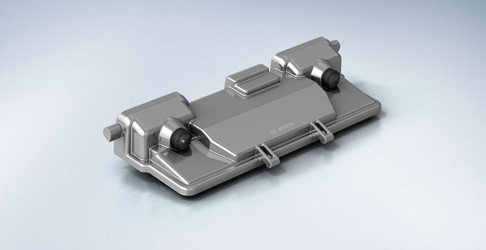
\includegraphics[width=0.8\textwidth]{chapters/images/svc}
  \caption{Bosch stereo camera}
\end{figure}

\subsubsection{Omni Camera}

The omni camera was an Allied Vision Technologies (AVT) Stingray camera, pair with an omni directional lense.  For the experiments performed, 1280x960 images with 8 bit depth were recorded at 30fps.  

The AVT camera is a generic camera, not specifically designed for omni-directional lenses and operates over a standard firewire 1394 interface.  As a result, the shutter and gain controls needed to be changed to ignore areas of the donut image with no data.  In this case the camera driver\footnote{ROS camera1394 package, \url{http://wiki.ros.org/camera1394}} was modified so that the calculation of the image brightness only considered valid pixels.

%These images were unwrapped to the circular images with a resolution of 2547x405.

\begin{figure}[H]
  \centering
    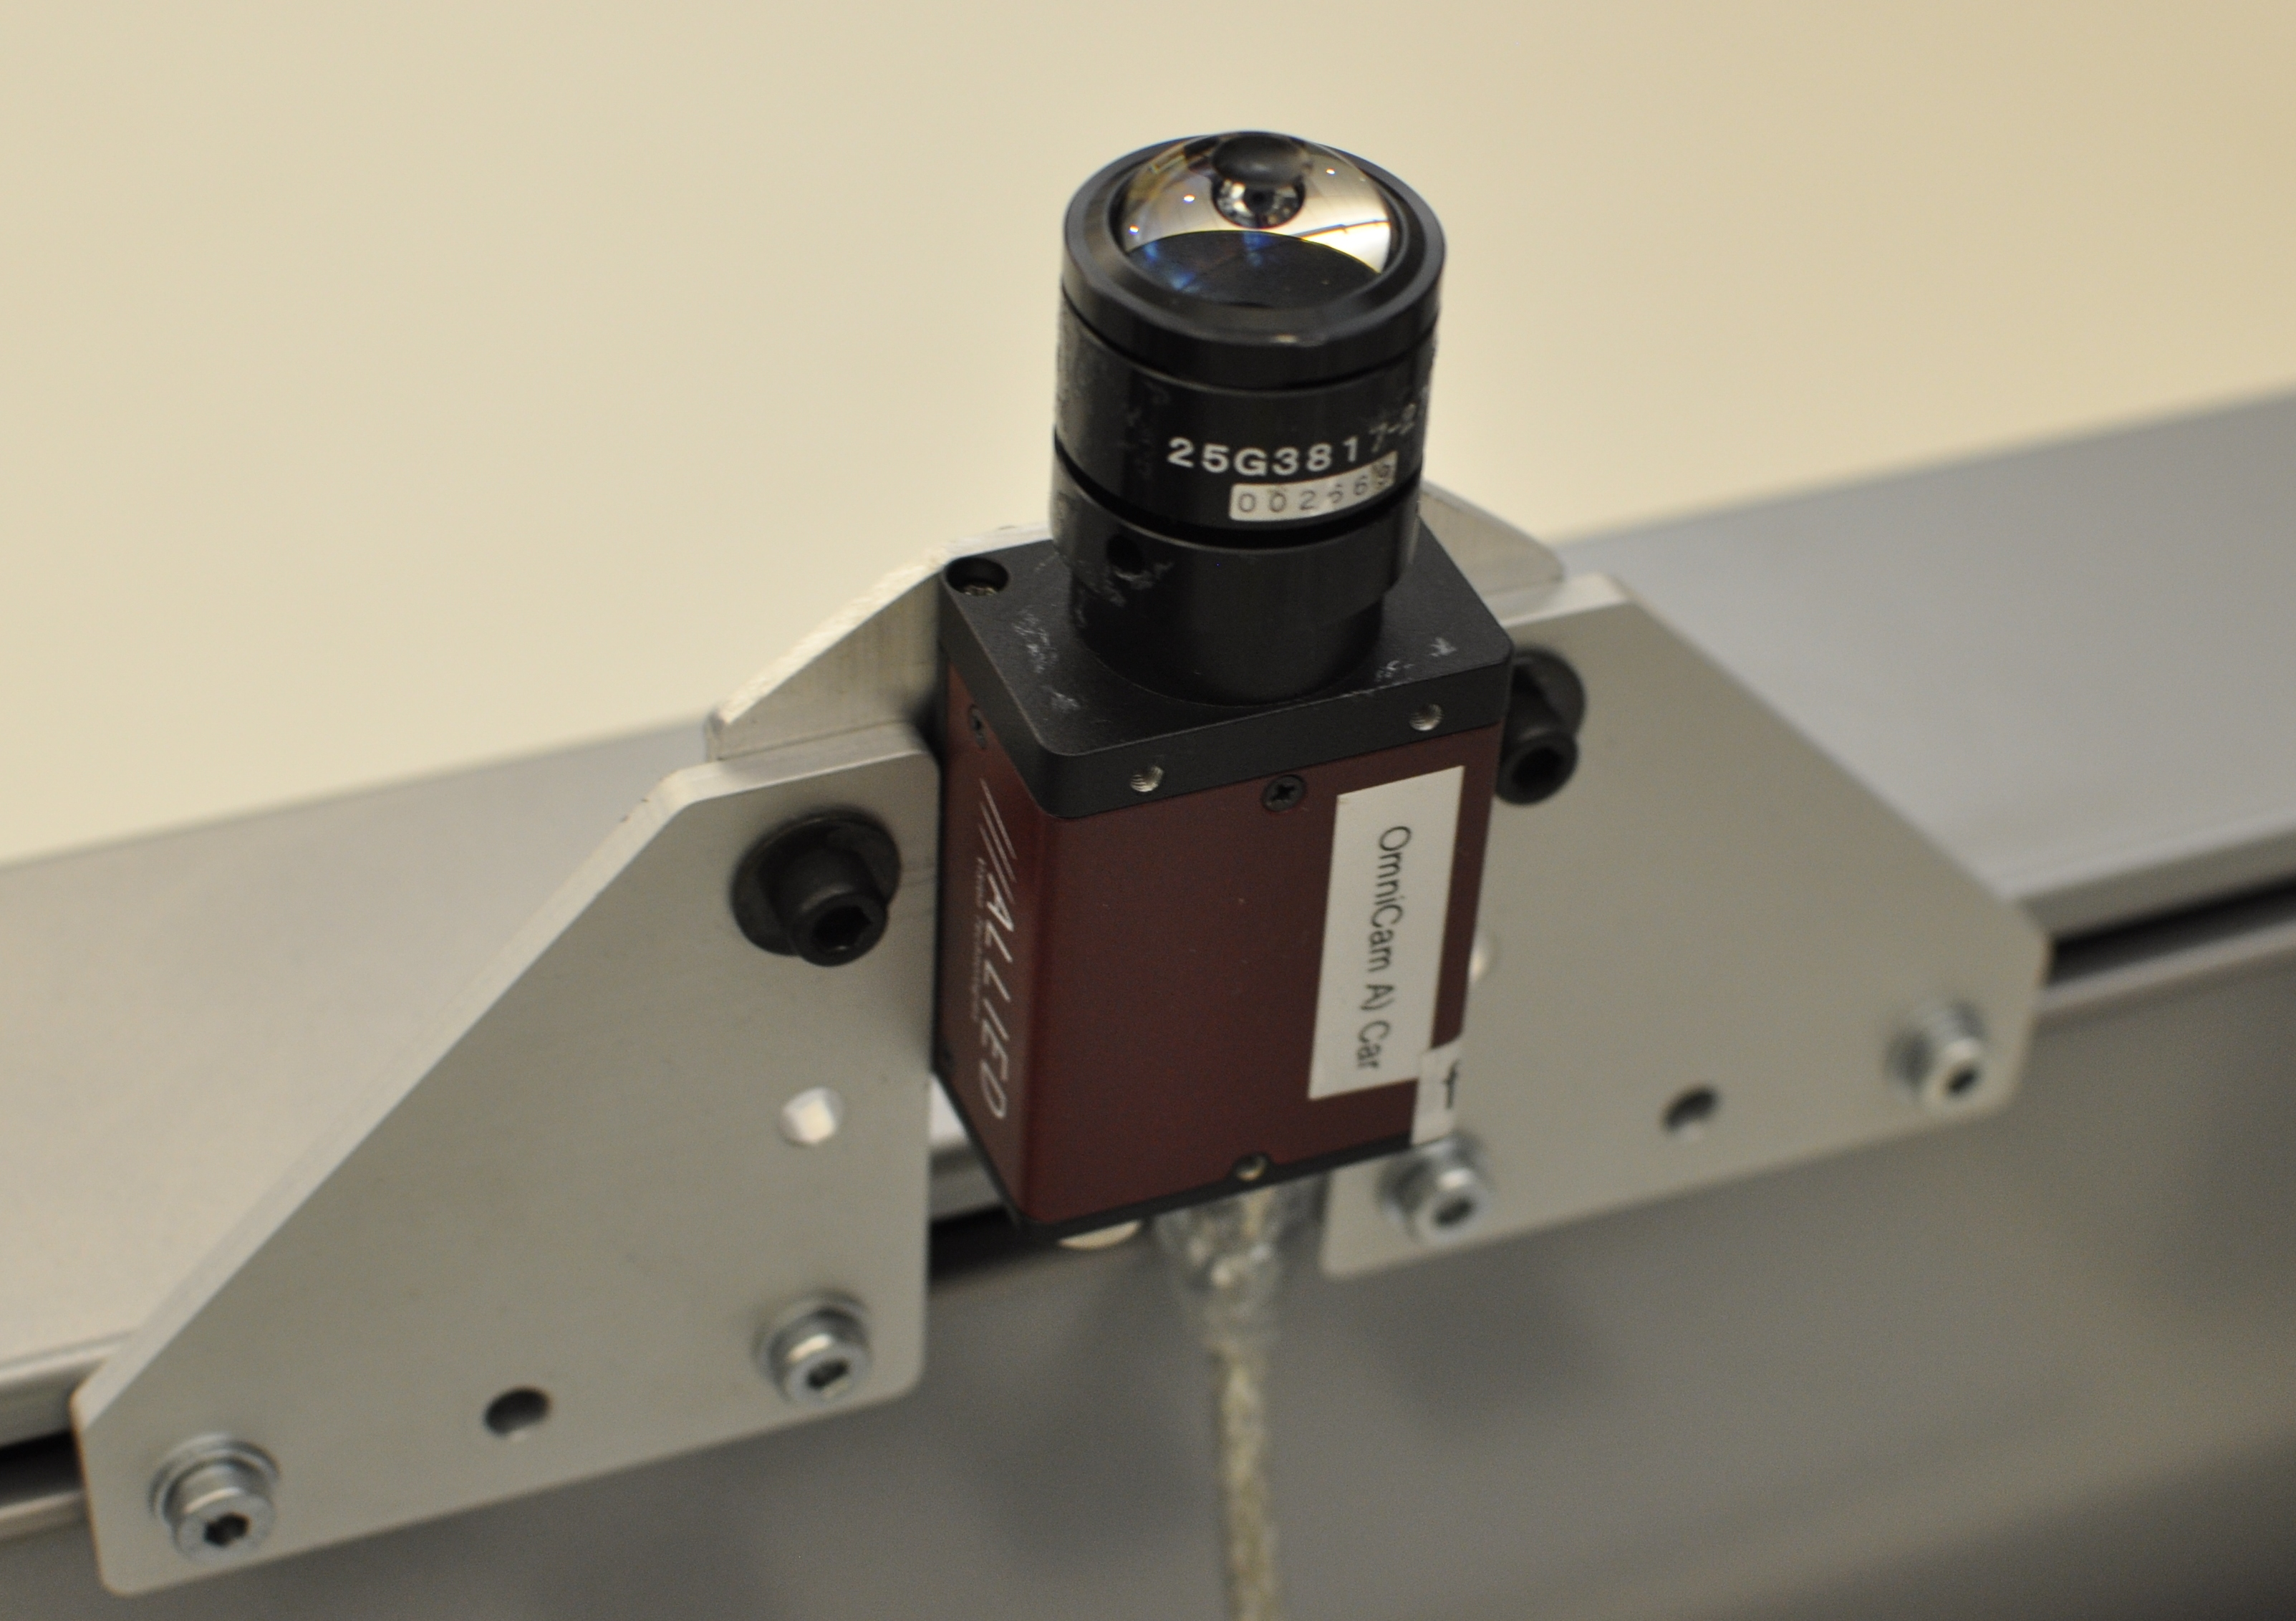
\includegraphics[width=0.5\textwidth]{chapters/images/omni_cam_image}
  \caption{AVT camera with Omni-directional lense and mounting brackets attached}
\end{figure}

\subsubsection{Camera Calibration}

Theory behind all the algorithms used is explained in Chapter \ref{chapter:extrinsic_calibration}, this section will describe the procedure undertaken.  The first step involved using the ROS calibration tool described in Section \ref{sec:ros_tool}.  This tool requires no initial condition to determine a calibration.  This was performed indoor with a checkerboard, but produced poor results because of the limited room to move the checkerboard around.

The calibration from the ROS calibration was used as an initial condition for the non linear optimization refinement. (See Section \ref{sec:g2o_extrinsic_cal}).  Video data was recorded outside using the online verification tool \ref{sec:verification_tool}.  In order to collect points of different depth, a textured surface was held in front of the camera at close range and moved slowly away.  Being outside, many distant points were also recorded.  The non linear extrinsic refinement tool was then run to obtain a refined calibration.   

\subsection{Groundtruth}

A combination of Differential Global Positional System (DGPS) and inertial sensors provided a ground truth trajectory poses (translation and rotation) with an accuracy of less than 50cm. 

\section{Evaluation Method}

The RGBD dataset tools\cite{sturm12iros} were used in order to evaluate error metrics on the trajectories generated by the modified ScaViSLAM system.  The RGBD dataset tools provide two metrics for evaluating trajectories; Absolute Trajectory Error (ATE) and Relative Pose Error (RPE).

\subsubsection{Relative Pose Error}

RPE is a measure of trajectory accuracy over some small fixed time interval.  In that sense it is a measure of drift.  If a trajectory to be evaluated is defined as $\bv P_1,....,\bv P_n \in \text{SE}(3)$ and the ground truth as $\bv Q_1,....,\bv Q_n \in \text{SE}(3)$ then the RPE at timestep $i$ may be defined as:

\begin{equation}
 \bv E_i := (\bv Q_i^{-1} \bv Q_{i+\Delta})^{-1}(\bv P_i^{-1} \bv P_{i+\Delta})
\end{equation}

The final root mean squared error (RMSE) over all time steps can be evaluated as:

\begin{equation}
 \text{RMSE}(\bv E_{1:n}) := \left( \dfrac{1}{m}\displaystyle\sum\limits_{i=1}^m \| trans(\bv E_i) \| ^2 \right)^\frac{1}{2}
 \label{eq:rmse}
\end{equation}

$trans()$ is a function taking only the translation component of the error and $m$ is total number all time intervals for a sequence of $n$ camera poses. 

This is a measure of drift, and is more applicable to visual odometry systems.  In this case the final SLAM graph trajectory after loop closures is of interest to us, not the visual odometry drift.  Loop closures should have little affect on the amount of drift in the SLAM system and therefore this method will not be used.

\subsubsection{Absolute Trajectory Error}

Absolute Trajectory Error evaluates how well an entire trajectory aligns to another one.  In order to compute this metric, first the trajectories need to be aligned as best as possible.  Horn\cite{Horn87} provides a closed form function to find the rigid body transformation $\bv S$ that performs this alignment of trajectory $\bv P$ onto ground truth trajectory $\bv Q$.  The error can then be computed for time step $i$ as follows:

\begin{equation}
 \bv E_i := \bv Q_i^{-1}\bv S \bv P_i
\end{equation}

The total RMSE can then be computed as per eq. \ref{eq:rmse}

The ATE provides a good measure of complete trajectory accuracy and therefore should be able to provide a good metric for if the loop closures provide an improvement to a trajectory.

\section{Experiments}

\subsection{Routes choose}

Two routes were selected for the evaluation.  The first 'two loops' dataset involved driving a small loop around two buildings, doing a three point turn, and then traversing the loop backwards to the start.  The idea behind this dataset is to not provide any chances for normal loop closures, whereby normal loop closures means the camera has a similar pose for both frames and the loop closure could be obtained with a standard stereo camera.  Therefor the omni-loop-closure pipeline should provide a very demonstrable improvement over the standard ScaViSLAM system.

The second route 'carpark loops', involves driving loops around 3 buildings and part of a carpark.  This provides a number of normal and opposite direction loop closures and therefore provides a longer evaluation sequence where the standard ScaViSLAM system should be able to perform well.

\begin{figure}[H]
  \centering
    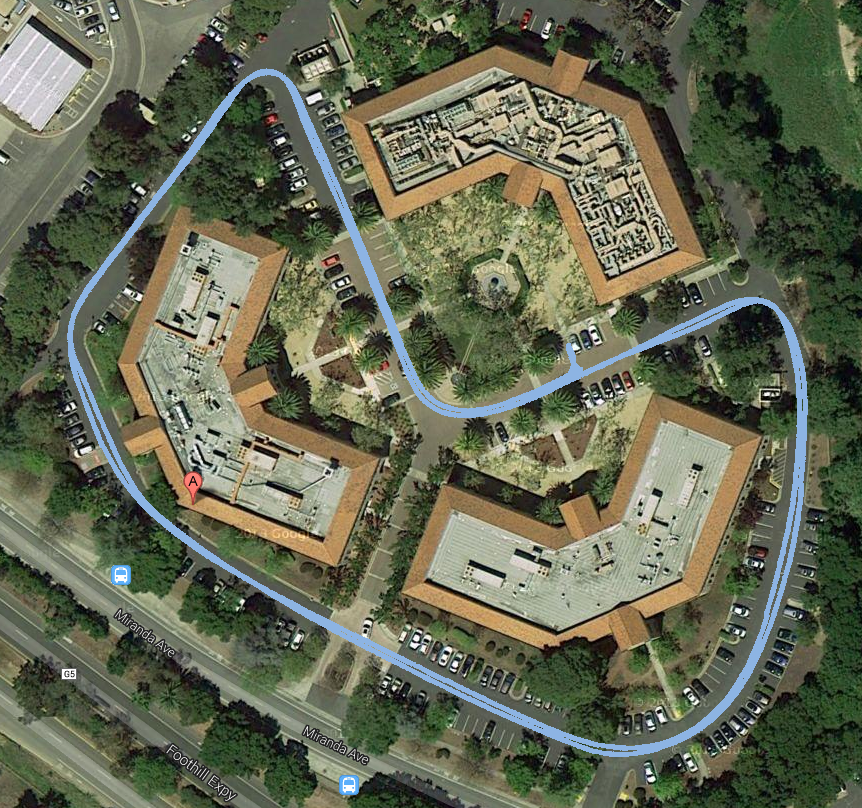
\includegraphics[width=0.5\textwidth]{chapters/images/two_loops_overlay}
  \caption{Overlay of the route on satellite imagery}
\end{figure}

\begin{itemize}
\item planned routes
\item driving conditions
\item size, time, length etc.
\end{itemize}

\subsection{Quantitative evaluation}

ATE is lower yay!

\subsection{Qualitative evaluation}

Look how much better the graphs are lol!

\subsection{Performance}

Min and max running times.  Caching of featuers, min run time important to increase number of tests.